\documentclass[a4paper,UKenglish]{lipics}

\usepackage[utf8]{inputenc}
% the following standard packages may be helpful, but are not required
%\usepackage{longtable}
\usepackage{mathtools}
\usepackage{multicol}
\usepackage{multirow}
\usepackage{booktabs}
\usepackage{courier}
\usepackage[scaled]{helvet}
\usepackage{url}
\usepackage{listings}
\usepackage{enumitem}
\usepackage{mdwlist} % tighter description environment (starred)

\usepackage{graphicx}
\usepackage{softdev}
\usepackage{amsmath}
\usepackage{mdwlist}
\usepackage{pifont}
\usepackage{xspace}

\newcommand{\kalibera}{Kalibera \& Jones\xspace}
\newcommand{\krun}{Krun\xspace}
\newcommand{\hypone}{H1\xspace}
\newcommand{\hyptwo}{H2\xspace}
\newcommand{\binarytrees}{\emph{binary trees}\xspace}
\newcommand{\richards}{\emph{Richards}\xspace}
\newcommand{\spectralnorm}{\emph{spectralnorm}\xspace}
\newcommand{\nbody}{\emph{n-body}\xspace}
\newcommand{\fasta}{\emph{fasta}\xspace}
\newcommand{\fannkuch}{\emph{fannkuch redux}\xspace}
\newcommand{\bencherthree}{Linux1/i7-4709K\xspace}
\newcommand{\bencherfive}{Linux2/i7-4790\xspace}
\newcommand{\benchersix}{OpenBSD/i7-4790\xspace}
\newcommand{\bencherseven}{ARM\edd{XXX name properly if used}\xspace}

\lstset{
    basicstyle=\tt\scriptsize,
    xleftmargin=2em,
    framexleftmargin=1.5em,
    numberstyle=\scriptsize\tt\color{gray},
    captionpos=b,
    escapeinside={{<!}{!>}},
}

\SDShowCommentTags{default}  %final

\begin{document}

\title{Virtual Machine Warmup Blows Hot and Cold}
\author[1]{Edd Barrett}
\affil[1]{Software Development Team, Department of Informatics,\\King's College London, \texttt{http://eddbarrett.co.uk/}}
\author[2]{Carl Friedrich Bolz}
\affil[2]{Software Development Team, Department of Informatics,\\King's College London, \texttt{http://cfbolz.de/}}
\author[3]{Rebecca Killick}
\affil[3]{Department of Mathematics and Statistics, University of Lancaster, \texttt{http://www.lancs.ac.uk/\~{}killick/}}
\author[4]{Vincent Knight}
\affil[4]{School of Mathematics, Cardiff University, \texttt{http://vknight.org/}}
\author[5]{Sarah Mount}
\affil[5]{Software Development Team, Department of Informatics\\King's College London, \texttt{http://snim2.org/}}
\author[6]{Laurence Tratt}
\affil[6]{Software Development Team, Department of Informatics\\King's College London, \texttt{http://tratt.net/laurie/}}

\Copyright{Edd Barrett, Carl Friedrich Bolz, Rebecca Killick, Vincent Knight, Sarah Mount and Laurence Tratt}
%\keywords{warmup, benchmarking, virtual machines, programming languages.}

% We need this to stop the running title from overflowing the margins.
\authorrunning{E. Barrett, C. F. Bolz, R. Killick, V. Knight, S. Mount, and L. Tratt}

\maketitle

\begin{abstract}
Virtual Machines (VMs) with Just-In-Time (JIT) compilers are traditionally thought
to execute programs in two phases: first the \emph{warmup} phase determines which
parts of a program would most benefit from dynamic compilation; after that
compilation has occurred the program is said to be at \emph{peak performance}.
When measuring the performance of JIT compiling VMs, data collected
during the warmup phase is generally discarded, placing the focus on peak
performance. In this paper we run a number of small,
deterministic benchmarks on a variety of well known VMs, showing a large number
of cases which fail to conform to the traditional notion of warmup. Indeed,
every VM we tested fails to conform to the traditional notion of warmup in at
least one benchmark, raising questions about how VMs should be benchmarked
\end{abstract}

\section{Introduction}
\label{sec:intro}

Many modern languages are implemented as Virtual Machines (VMs) which use a
Just-In-Time (JIT) compiler to translate `hot' parts of a program into efficient
machine code at run-time. Since it takes time to determine which parts of the
program are hot, and then compile them, programs which are JIT compiled are
said to be subject to a \emph{warmup} phase. The traditional view of
JIT compiled VMs is that program execution is slow during the warmup phase, and
fast afterwards, when \emph{peak performance} is said to have been reached
(see Figure~\ref{fig:trad} for a simplified view of this).
This traditional view underlies most benchmarking of JIT compiled VMs, which
generally aim to measure peak performance.
Benchmarking methodologies usually
require running benchmarks several times within a single VM process, and
discarding any timing data collected before warmup is complete.

Our fundamental aim in this paper is to test the following hypothesis, which captures a constrained
notion of the traditional notion of warmup:
\begin{description}
  \item[\hypone] Small, deterministic programs exhibit traditional warmup behaviour.
\end{description}
In order to test this hypothesis, we present a carefully designed
experiment where a number of simple benchmarks are run on a variety of
VMs for a large number of \emph{in-process iterations} and repeated using fresh
\emph{process executions} (i.e.~each process execution runs multiple in-process
iterations). Note that we deliberately treat VMs as black
boxes: we simply run benchmarks and record timing data. It is not our intention
to understand the effects we see in the resulting timing data, for the simple
reason that we are not experts in most of the VMs under investigation. Even were
we experts, understanding some of the resulting data could take many person
months of effort per VM.
%From this we obtain \emph{time series} data, to which we apply a
%number of statistical techniques that have not previously been applied
%in the context of VM benchmarking.

\begin{figure}[t]
\centering
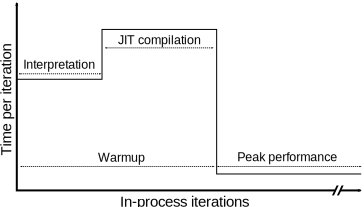
\includegraphics[width=.5\textwidth]{img/picturebook_warmup}
\caption{The traditional notion of warmup: a program starts slowly executing in
an interpreter; once hot parts of the program are identified, they are
translated by the JIT compiler to machine code; at this point warmup
is said to have completed, and peak performance reached.}
\label{fig:trad}
\end{figure}

We expected our experiment to validate Hypothesis H1, allowing us to
easily compare warmup across VMs. While some benchmarks on some VMs run as per
traditional expectations, we found a number of surprising cases. At
the most extreme, some benchmarks never warm up, staying at their initial performance
levels indefinitely and some even slowdown. Even for
those benchmarks that appear to warm up in a traditional fashion, there are
various performance patterns that make presenting a simple performance number
difficult. Of the eight VMs we looked at,
none consistently warmed under the traditional model.

Our results clearly show that the traditional view of warmup is no longer valid (and, perhaps,
that it may not have held in the past). We are not aware that anyone has systematically noted this
problem before, let alone take it into account when benchmarking. This suggests
that many published VM benchmarks (including our own) may have presented
results which are misleading in some situations.

A reasonable question is whether inaccuracies in VM benchmarking are of anything
other than academic interest. We believe that accurate VM benchmarking is needed
by both VM authors and many end users. When
implementing optimisations, VM authors need to know if their optimisations have
had the intended effect or not: since many optimisations, in isolation, have only a
small effect, accurate benchmarking is vital. Our results suggest that decisions
about the effectiveness of an optimisation may sometimes be made based on
incomplete, and thus unreliable, data; 
it is likely that this has caused some ineffective, and perhaps even some deleterious,
optimisations to included in VMs. Many end users have workloads that are more
sensitive to latency than throughput. For example, users running games (or other
soft real-time systems) require predictable performance. Our results show that some
VMs JIT compile programs that have unpredictable long-term performance.

%This paper's contributions are as follows:
%\begin{enumerate*}
%  \item \laurie{blah blah}
%\end{enumerate*}
%
%This paper's structure is as follows. \laurie{blah blah}


\section{Background}
\label{sec:warmup}

When a program begins running on a JIT compiled VM, it is typically (slowly)
interpreted; once `hot' (i.e.~frequently executed) loops or methods are
identified, they are dynamically compiled into machine code; and subsequent
executions of those loops or methods use (fast) machine code rather than the
(slow) interpreter. Once machine code generation has completed, the VM is
traditionally said to have finished warming up, and the program to be executing
at peak performance.\footnote{This traditional notion applies equally to VMs
that perform immediate compilation instead of using an interpreter, and to
those VMs which have more than one layer of JIT compilation (later JIT
compilation is used for `very hot' portions of a program, and tolerates slower
compilation time for better machine code generation).}

Figure~\ref{fig:trad} shows the expected performance profile of a
program subject to the conventional model of warmup. Exactly how long warmup
takes is highly dependent on
the program and the JIT compiler, but this basic assumption about the
performance model is shared by every JIT compiling
VM~\cite{kalibera13rigorous}.

Benchmarking of JIT compiled VMs typically focusses on peak
performance. The
methodologies used are typically straightforward: benchmarks are run for a number
of in-process iterations within a single VM process execution.
The first $n$ in-process iterations are then discarded, on the basis that warmup
will have completed at some point before $n$. It is common for
$n$ to be a hard-coded number -- in our experience it is often set at 5 --
that is used for all benchmarks.

One of the obvious flaws in this simple methodology is that one does not know if warmup
has completed by in-process iteration $n$. A more sophisticated VM benchmarking methodology
was developed by \kalibera to solve a number of issues when benchmarking JIT
compiling VMs~\cite{kalibera12quantifying,kalibera13rigorous}. The basic idea is
that, for a given VM / benchmark combination, a human must inspect the data from
executing a small number of VM process executions, and determine at which in-process iteration the
benchmark has definitively warmed up. A larger number of VM process executions are then
run, and the previously determined cut-off point applied to each process's
iterations. The \kalibera methodology observes that some benchmarks do not
obviously warm up; and that others follow cyclic patterns post-warmup
(e.g.~in-process iteration $m$ is slow, $m+1$ is fast, for all even values of $m > n$). In
the latter case, the \kalibera methodology requires a consistent in-process iteration in
the cycle to be picked for all process executions, and that used for statistical analysis.

To the best of our knowledge, the \kalibera methodology is the most
sophisticated currently available (see its use in
e.g.~\cite{barrett15approaches,grimmer15dynamically}). While the \kalibera
methodology is a real improvement over straightforward benchmarking methodologies,
our experience has been that there remain cases where it remains hard to produce
satisfying benchmarking statistics. Crucially, the methodology does not
provide a firm way of determining when warmup has completed. Because of this
``determining when a system has warmed up, or even providing a
rigorous definition of the term, is an open research problem''~\cite{seaton15phd}.


\section{Methodology}
\label{sec:methodology}

To test Hypothesis H1, we designed an experiment which uses a suite of
micro-benchmarks: each is run with 2000 in-process iterations and repeated
using 10 process executions. So as
to collect high-quality data, we have carefully designed our
experiment to be repeatable and to control as many potentially confounding variables as
is practical.

In this section we detail: the benchmarks we used and the modifications we
applied; the machines we used for benchmarking; the VMs we benchmarked; and the
\krun system we developed to run benchmarks.


\subsection{The Micro-benchmarks}

The micro-benchmarks we use are as follows: \binarytrees, \spectralnorm, \nbody,
\fasta, and \fannkuch from the Computer Language Benchmarks Game (CLBG); and
\richards. Readers can be forgiven for initial scepticism about this set of micro-benchmarks.
They are small and widely
used by VM authors as optimisation targets. In general they are more effectively
optimised by VMs than average programs; when used as a proxy for other types
of programs (e.g.~large programs), they tend to overstate the effectiveness of
VM optimisations. In our context, this weakness is in fact a strength: we need
small, deterministic, and widely examined programs so that we can test
Hypothesis \hypone. Put another way, if we were to run arbitrary programs
and find unusual warmup behaviour, a VM author might reasonably counter that
``you have found the one program that exhibits unusual warmup behaviour''.

For each benchmark, we provide C, Java, Javascript, Python, Lua, PHP,
and Ruby versions.\footnote{Our need to have implementations in a wide variety
of languages restricted the micro-benchmarks we could use.} Since most of these
benchmarks have multiple implementations in any given language, we picked
the same versions used in~\cite{bolz14impact}, which represented the fastest
performers at the point of that publication. We were forced to skip some
benchmark and VM pairings which either ran prohibitively slowly
(Fasta/JRubyTruffle and Richards/HHVM), or caused the VM to crash
(SpectralNorm/JRubyTruffle).\footnote{Later versions of this paper
will use newer VM versions, which we hope may fix these problems.}
For the avoidance of doubt we
did not interfere with any VM's Garbage Collection (GC) (e.g.~we did not
force a collection after each iteration).


\subsubsection{Ensuring Determinism}

We wish to ensure, as far as possible, that the micro-benchmarks are
deterministic from the user's perspective, by which we mean that they
take precisely the same path through the Control Flow Graph (CFG) on each
execution and iteration. Note that this definition deliberately focuses
on non-determinism that is controllable by the user; other forms of
non-determinism within the VM are deliberately excluded, as they are
part of what we are trying to measure (e.g.~objects in memory may be allocated
or garbage collected non-deterministically). To test this, we created variants
of all benchmarks with \texttt{print} statements at all possible points of
divergence (e.g.~\texttt{if} statements' true and false branches). These
variants are available in our experimental suite.

We first ran the benchmarks with 2 process executions and 20 in-process iterations,
and compared the outputs of the two processes. This was enough to show that the
\fasta benchmark was non-deterministic
in all language variants. This is because \fasta generates random numbers with
a seed that is initialised only at the very start of the benchmark, thus
causing each in-process iteration to generate different random numbers. We
fixed this by moving the random seed initialisation to the start
of the in-process iteration main loop.

Bearing in mind surprising
results such as the importance of link order~\cite{mytkowicz09surprising}, we
then used two different machines to compile VMs and then ran the benchmarks
on these machines.
Using this technique we noticed occasional non-determinism in Java benchmarks.
This ultimately turned out to be caused by lazy class loading. In order
to make our benchmarks run well with \krun (see Section~\ref{krun}), we
altered them such that each has an additional \texttt{KrunEntry} class,
which, in essence, provides an interface between \krun and the main benchmark
class. Because of this, the main benchmark class was lazily loaded after
benchmark timing had started (sometimes in a way that we could observe). We
solved this by adding to each benchmark an empty static method, which each
\texttt{KrunEntry} then calls via a static initialiser. In so doing, we
guarantee that the main benchmark class is not lazily loaded. Note that Java
benchmarks -- as well as
Java-based systems such as Graal and JRuby/Truffle -- will still be subject to
lazy loading, which is an inherent part of the JVM specification: forcing all
classes to be eagerly loaded is impractical, and is thus part of the warmup we
wish to measure.


\subsection{Measuring Computation and Not File Performance}

Micro-benchmarks often perform computations which are partly or wholly irrelevant. Highly
optimising compilers are thus often able optimise away part or all of a
micro-benchmark's computation. In one sense, this is a desirable part of
optimising compilers~\cite{seaton15phd}, though benchmarks whose computations
are entirely removed are rarely useful. To ensure that computation cannot
be optimised away, many benchmarks write intermediate and final results
to \texttt{stdout}. However, one can quickly end up in a situation where benchmarks are
unintentionally measuring, in part or whole, the performance of file routines in
the OS libraries and the kernel.

To avoid both of these unfortunate cases,
we modified the benchmarks to calculate a checksum during each in-process iteration.
The checksum is validated at the end of each in-process iteration against an expected
value; if the check fails, the incorrect checksum is written to \texttt{stdout}.
By writing benchmarks in
this style, we make it difficult for optimising compilers to remove the
main bulk of the benchmark. Note that each micro-benchmark has a single checksum value for all
language variants, which also provides some assurance that each language variant is
performing the same work.


\subsection{Benchmarking Hardware}

%We used three machines and two operating systems:
We used two benchmarking machines:

\begin{tabular}{ll}
  \bencherthree & Quad-core i7-4790K 4GHz, 24GB of RAM, running Debian 8. \\
  \bencherfive  & Quad-core i7-4790 3.6GHz, 32GB of RAM, running Debian 8.
%  \item[\benchersix] Identical hardware to \bencherfive, but running OpenBSD 5.8.
\end{tabular}

\noindent These machines allow us to investigate the effects of moderately different
hardware (\bencherthree and \bencherfive run the same operating system with the
same updates installed)
%as well as moderately different operating systems
%(\bencherfive and \benchersix have almost identical hardware, but run different
%Unix
%variants). With regards to hardware and operating systems, we started with the
%following hypothesis:
%\begin{description}
%  \item[\hyptwo] Moderately different hardware and operating systems have little effect on warmup patterns.
%\end{description}
%We deliberately use the word `moderately', since significant changes of hardware
%(e.g.~x86 vs.~ARM) or operating system (e.g.~Linux vs.~Windows) implies that
%significantly different parts of the VMs will be used (e.g.~different machine
%code backends may be of differing levels of maturity).

We disabled turbo boost and hyper-threading in the BIOS. Turbo boost is a
feature which allows CPUs to temporarily run in an extremely high-performance
mode; this eventually causes the CPU to exceed its safe thermal limit,
at which point it reduces performance it has cooled down sufficiently.
Turbo boost can thus cause long-running processes to
appear to suddenly slow down. Hyper-threading gives the illusion that a single
physical core is in fact more than one logical core, inter-leaving the
execution of two or more programs or threads on a single physical core.
Hyper-threading causes programs to interfere
with each others in complex ways, introducing considerable noise. It
is of no real benefit in our situation, where we do not make use all of the
physical cores in our benchmarking machines.


\subsection{VMs under investigation}

We ran the benchmarks on the following language implementations:

\begin{tabular}{ll}
GCC & Version 4.9.2 (from Debian packages). \\
Graal \#9dafd1dc5ff9 & HotSpot using a next-gen compiler. \\
HHVM 3.7.1 & A PHP JIT compiled VM. \\
JRuby/Truffle \#7f4cd59cdd1c8 & A Ruby interpreter using Graal for compilation. \\
HotSpot 8u45b14 & The most widely used Java VM. \\
LuaJIT 2.0.4 & A tracing JIT compiler for Lua. \\
PyPy 4.0.0 & A meta-tracing VM for Python 2.7. \\
V8 4.8.271.9 & A JIT compiler for Javascript.
\end{tabular}
\edd[final]{Add to list: CPython 2.7.10, The reference Python implementation}%

\noindent Although not a VM, GCC serves as a baseline to compare the VMs against.

We created a build script which downloads, configures, and builds fixed
versions of the
VMs, ensuring we can easily repeat builds.
All VMs were compiled with GCC/G++ 4.9.2.\edd[final]{Say something about a
fixed GCC accross platforms}\edd[final]{Neither HHVM nor
JRuby/Truffle has currently been ported to OpenBSD, and thus we were unable to
run those VMs on OpenBSD.}


\subsection{\krun}
\label{krun}

We developed a tool called \krun to fully automate the running of benchmarks
and to control the environment under which the benchmarks run. \krun itself is a
`supervisor' process which first configures a system before running VM-specific
benchmarks, monitoring the system for any signs of errors during benchmarking,
and writing results to a compressed JSON file. \krun is invoked with a
configuration file which describes the VMs, benchmarks, and number of process
executions and in-process iterations to
be executed.

In the remainder of this subsection, we describe: the variables which \krun
controls (both generic and platform dependent); and how \krun collects data.
Note that, although \krun has `developer' modes which disable various checks,
we describe only the `production' mode, which has all checks enabled.


\subsubsection{Platform Independent Controls}

Several of \krun's controls work on all supported platforms. \krun imposes a
consistent heap and stack \texttt{ulimit} for all
VMs (we used a 2GiB heap and a 8MiB stack).\footnote{Note that Linux allows users
to inspect these values, but to allocate memory beyond them.} Benchmarks are run
as the Unix user `\texttt{krun}', which performs no environment configuration.
\krun reboots the system before each process execution (including
before the first) to ensure that the system is in a somewhat known state
(e.g.~if a benchmark caused a system to transfer memory from RAM to disk-based swap,
rebooting ensures that later benchmarks are not affected). After each reboot, \krun
is invoked automatically by the system's init subsystem; it pauses for 3 minutes to allow the system
to fully initialise before running the next process execution.

\krun performs two types of monitoring before and during benchmark execution.
First, \krun monitors the system's \texttt{dmesg} buffer, informing the user of
any changes. We implemented this feature after noticing that one of the
machines we had earlier ear-marked for running benchmarks occasionally
overheated, with the only clue to this being a message left in the \texttt{dmesg}.
We did not use this machine for our final benchmarking.
Second, \krun monitors temperature sensors. Since modern systems may limit
performance when they get too hot, \krun ensures that all process executions
start at approximately the same temperature. When benchmarking commences,
\krun waits for a fixed period of time (60s) in the hope that the machine
cools down.; after this point, it collects temperature
readings from all available temperature sensors, which are then used as
the base temperature readings. Before each subsequent process execution, \krun
waits until the temperature sensors are within 10\%{} of the base temperatures
before continuing. If any sensor fails to meet this threshold
within 10 minutes, \krun terminates the entire experiment.


\subsubsection{Linux-specific Controls}

On Linux, \krun controls several additional factors.

\krun sets the CPU frequency to the highest non-over-clocked value possible.
The user must first disable Intel P-state support in
the kernel by passing the kernel argument \texttt{intel\_pstate=disable}.
\krun verifies P-states are disabled and uses \texttt{cpufreq-set} to set
the CPU governor to \texttt{performance} mode. Note that even with these
options set, we cannot fully guarantee that the CPU does as requested
(see Section~\ref{sec:threats} for details).

\krun checks that it is running on a `tickless' kernel, which aims to reduce
jitter in time-sensitive workloads~\cite{tickless}. The default
Linux kernel interrupts each active logical CPU\footnote{Note that each core of
each individual processor chip counts as a logical CPU.} 250 times (`ticks') a second to
decide whether to perform a context switch. We used a kernel with the
\texttt{CONFIG\_NO\_HZ\_FULL\_ALL} compile-time option set, which puts
all CPUs except one (the boot CPU) into adaptive-tick mode.
CPUs in adaptive-tick mode are only interrupted by the kernel if more than
one runnable process is scheduled.
When we compared a subset of benchmarks on a tickless vs.~a standard
kernel, we noticed a small reduction in jitter, although not enough for us to
conclusively say that the tickless kernel was the cause. However,
since, at worst, it appears to have no negative effects, we ran our experiments
using the tickless kernel.

Linux's \texttt{perf} system dynamically profiles system performance by
repeatedly sampling hardware counters. We became aware of \texttt{perf} when
\krun's \texttt{dmesg} checks notified us that the kernel had decreased the
sample-rate as it determined that it was sampling too often. Since \texttt{perf}
can interrupt benchmarking, its existence is undesirable, particularly since its
effects can vary over time. Although \texttt{perf} cannot be disabled entirely,
\krun sets the sample-rate to the smallest possible value of 1 sample per
second.

Finally, \krun disables Address Space Layout Randomisation (ASLR). While this is
a sensible security precaution for everyday use, it makes it difficult to
compare the performance of even a single binary.\footnote{The Stabilizer
system~\cite{curtsinger13stabilizer} is an intriguing approach for obtaining reliable
statistics in the face of features such as ASLR. Unfortunately we were not able
to build it on a modern Linux system.} \krun sets the
\texttt{randomize\_va\_space} entry in \texttt{/proc} to 0, disabling ASLR
globally.


%\subsubsection{OpenBSD-specific Controls}
%
%Relative to Linux, OpenBSD exposes many fewer knobs to users. Nevertheless,
%there are two OpenBSD specific features in \krun.
%
%First, \krun sets CPU performance to maximum by invoking \texttt{apm -H} prior
%to running benchmarks. This is equivalent to setting Linux's CPU governor to
%\texttt{performance} mode, but note that OpenBSD offers no means of changing
%Intel P-states.
%
%Second, \krun sets OpenBSD's default \texttt{malloc} implementation to be
%deterministic. By default, OpenBSD's \texttt{malloc} performs several operations
%for security purposes, including allocating guard pages and randomising layout.
%We set the \texttt{MALLOC\_OPTIONS} environment variable to \texttt{sfghjpru},
%turning it into a more traditional, and hopefully largely deterministic,
%\texttt{malloc}.


\subsubsection{The Iterations Runners}

Since we run benchmarks in several different languages, we need a way to report
timings from benchmarks to \krun. For each language, we created an
\emph{in-process iterations runner}. When \krun wants to run a benchmark, it executes the
appropriate in-process iterations runner for that language, passing it the name of the
benchmark to be run, and the desired number of in-process iterations. The in-process iterations runner
then dynamically loads the benchmark, and repeatedly executes the main body of
the benchmark. The in-process iterations runner calls a monotonic timer with
sub-millisecond accuracy before and after each iteration, recording the result
into a list; when the iterations are complete, it returns the results
to \krun by printing a JSON list to stdout.

Most VMs and languages expose access to the low-level monotonic timing
\texttt{clock\_gettime} function as standard. We extended V8, HHVM and JRuby/Truffle
to expose this monotonic clock via a user-visible function.
%On OpenBSD, we use
%the \texttt{CLOCK\_MONOTONIC} timer; on Linux this timer is subject to
%interference from the \texttt{adjtime} function, and we thus use the
%\texttt{CLOCK\_MONOTONIC\_RAW} timer.


\section{Classifying Results}
\label{sec:Results}

Our experiment runs 450 unique process executions, giving a total of 900\,000
in-process iteration readings. For each process execution we generate a
run-sequence graph, with in-process iterations on the $x$ axis, and the time
per in-process iteration on the $y$ axis.
These graphs, though simple, highlight a number of
interesting features, which we informally classify.

One common feature in our results are \emph{outliers}: informally, these are
in-process iterations which are slower (or, less commonly, much
faster) than neighbouring in-process iterations. In general, we disregard outliers
when classifying data (i.e.~we pretend the outliers do not exist). Figure~\ref{fig:examples:outliers1}
shows a typical
example, where in amongst largely consistent timings, a single in-process
iteration is substantially slower than its neighbours.


\begin{figure}[tbp]
\makebox[\textwidth][c]{
\begin{minipage}{.65\textwidth}
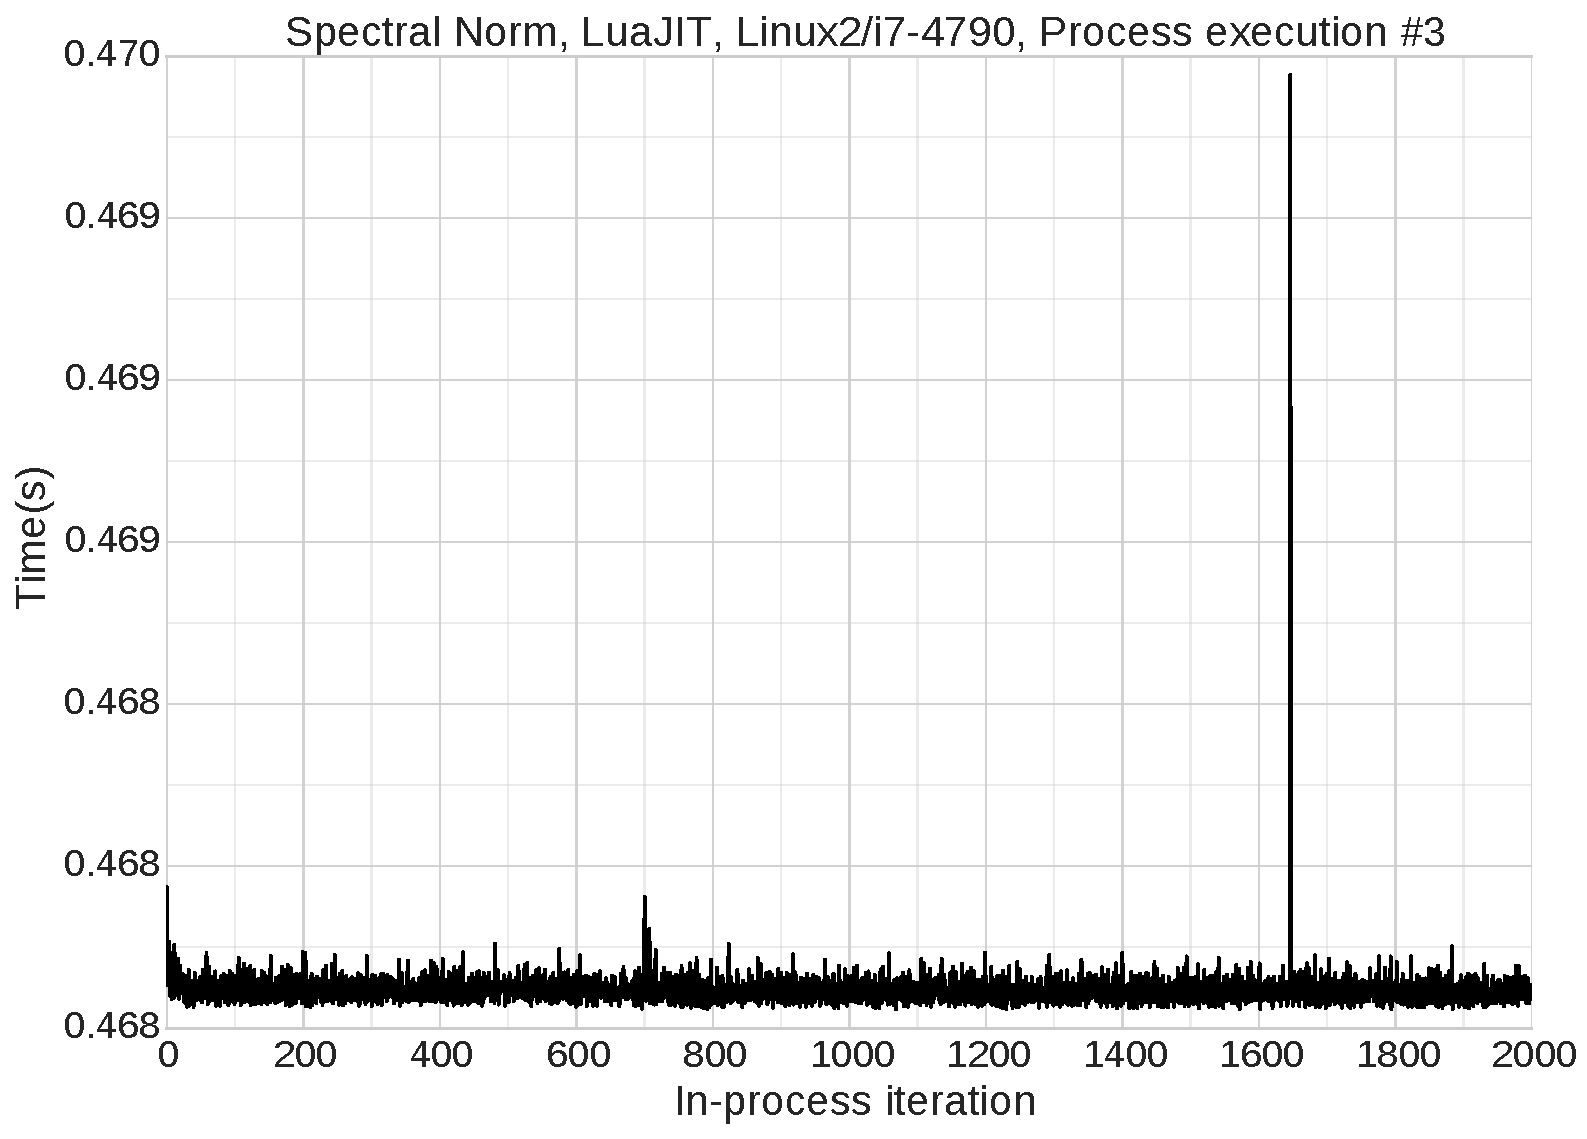
\includegraphics[width=\textwidth]{examples/outliers1}
\end{minipage}
}
\caption{A process execution with an outlier at in-process iteration \#1646.}
\label{fig:examples:outliers1}
\end{figure}


\subsection{Classifications}

Our classifications are as follows.

\begin{figure*}[tbp]
\makebox[\textwidth][c]{
\begin{minipage}{.65\textwidth}
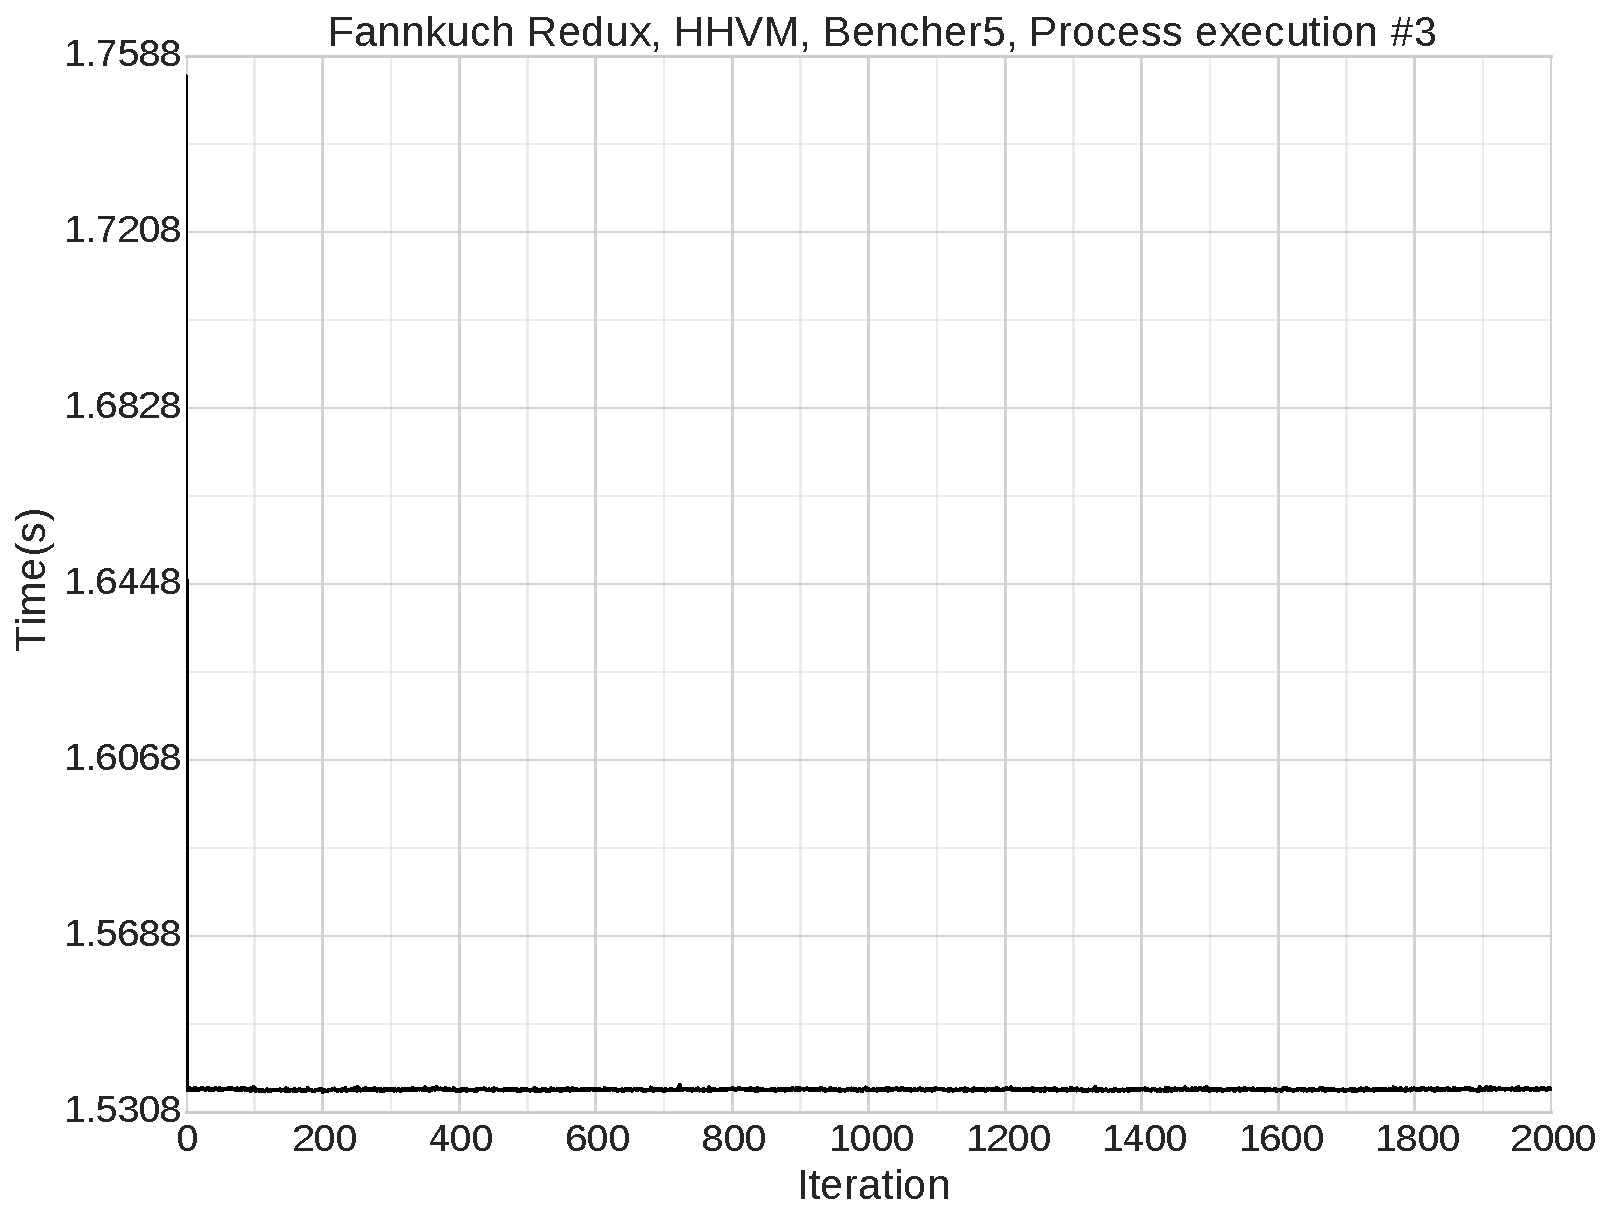
\includegraphics[width=\textwidth]{examples/good1.pdf}
\end{minipage}
\begin{minipage}{.65\textwidth}
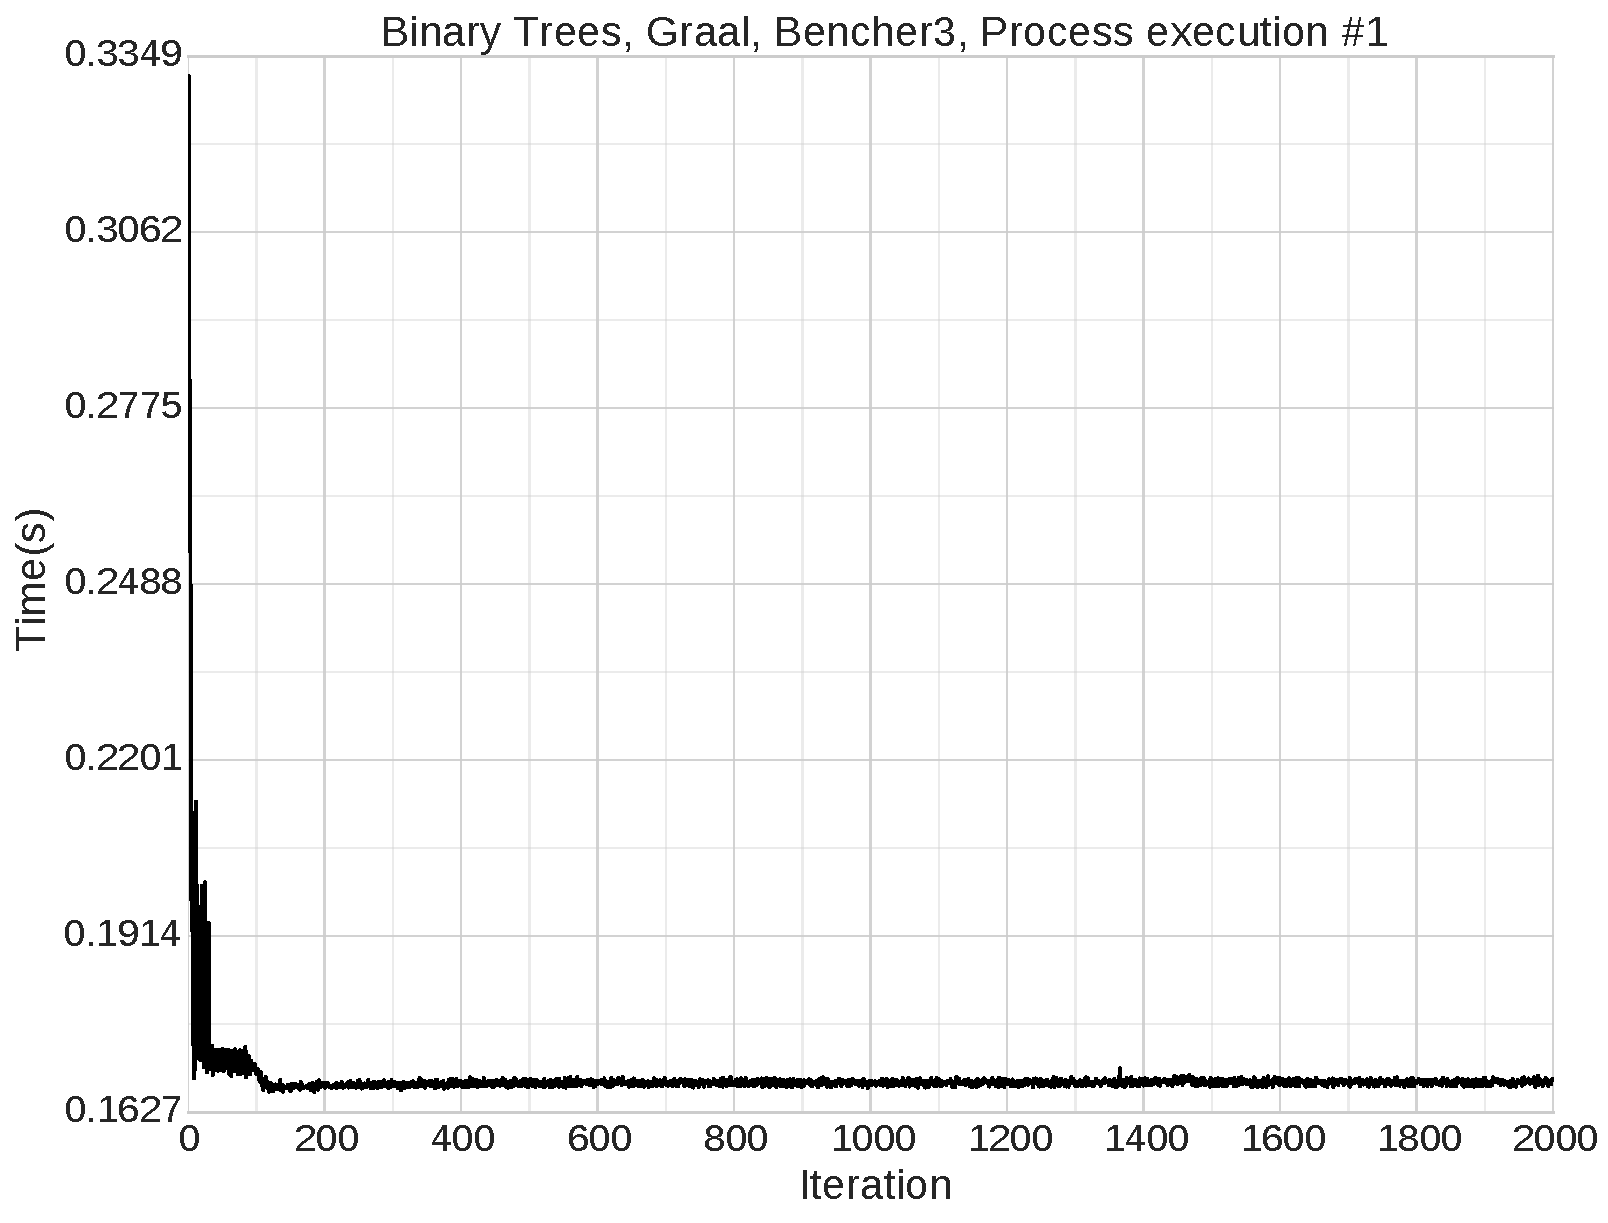
\includegraphics[width=\textwidth]{examples/good2.pdf}
\end{minipage}
}
\caption{Two examples of traditional, warmup behaviour. On the left-hand side,
warmup is complete by in-process iteration 1; on the right-hand side by around
iteration \#120.}
\label{fig:examples:trad}
\end{figure*}

\textbf{Traditional Warmup} Of the 39 benchmark/VM pairs we ran, less than 10
could be said to \emph{consistently} warm-up as per traditional
expectations.\footnote{Giving a precise number is tricky, as without a formal
definitions, our classifications are largely open to interpretation.}
Figure~\ref{fig:examples:trad} shows examples of process executions that
warm-up as expected.


\begin{figure}[tbp]
\makebox[\textwidth][c]{
\begin{minipage}{.65\textwidth}
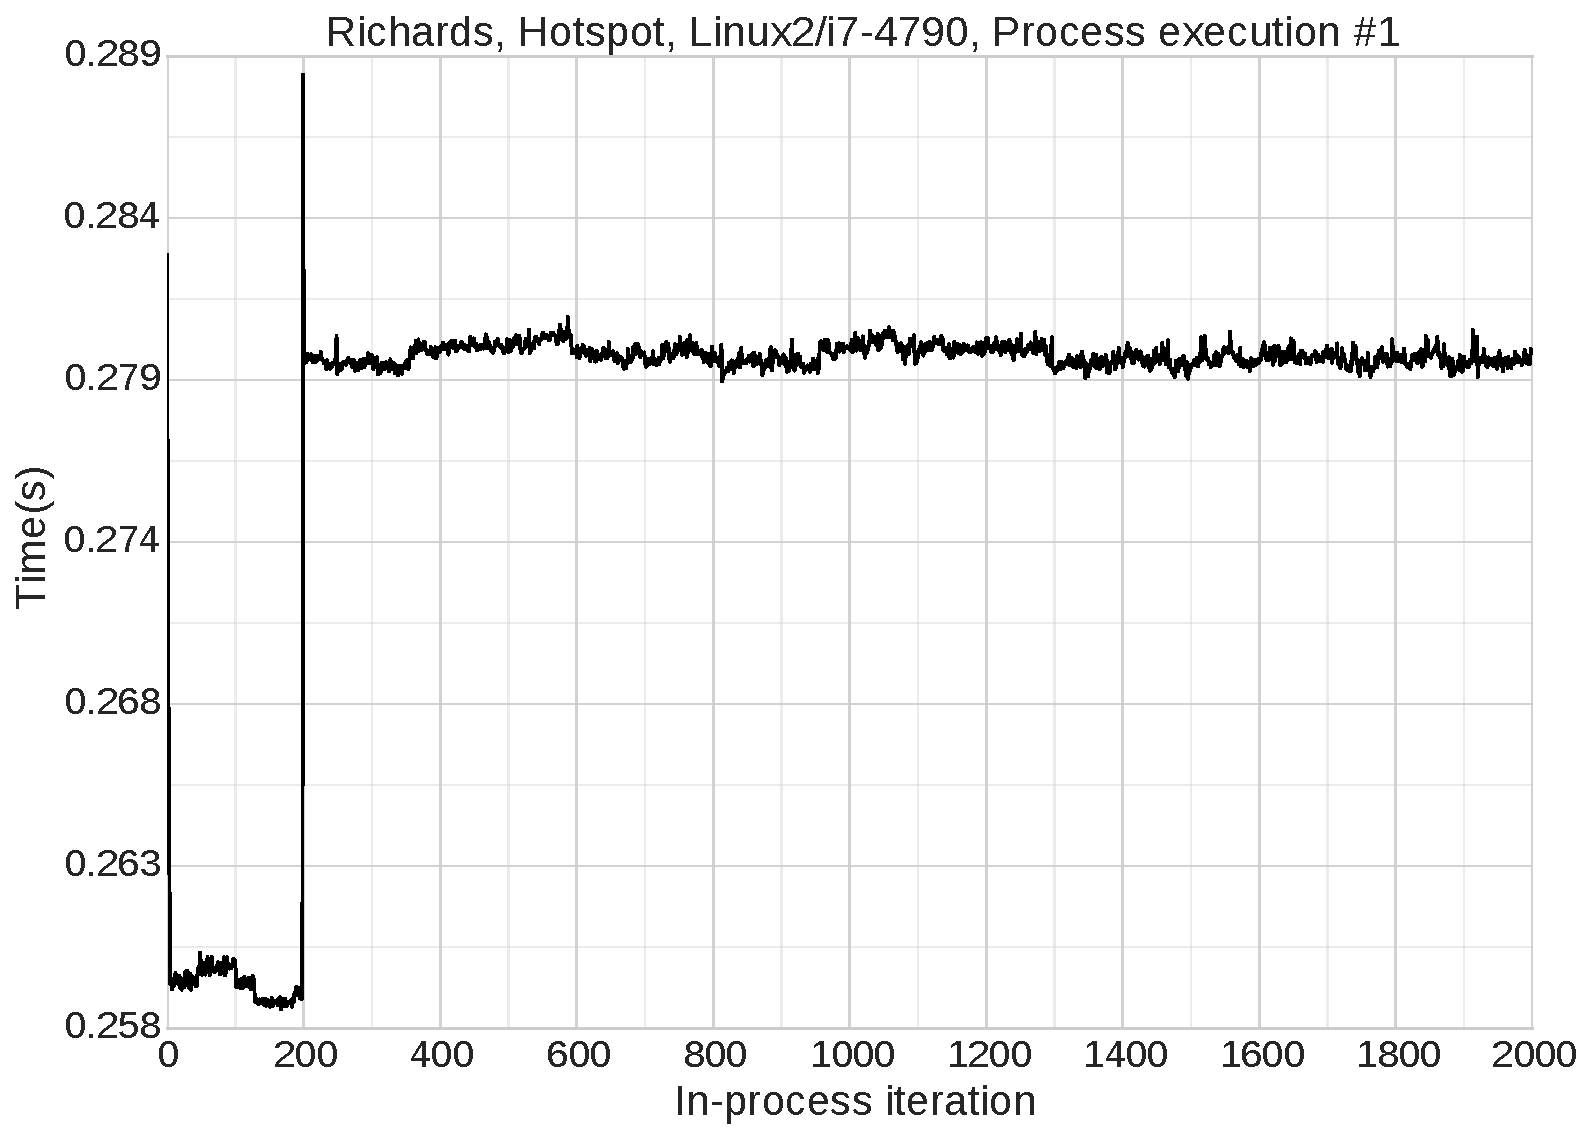
\includegraphics[width=\textwidth]{examples/slowdown1}
\end{minipage}
}
\caption{An example of slowdown, occurring at in-process iteration \#199.}
\label{fig:examples:slowdown1}
\end{figure}

\textbf{Slowdown} \label{sub:slowdowns}
In stark contrast to the traditional expectation of `warmup', some benchmarks
exhibit `slowdown', where the performance of
in-process iterations drops over time. Figure~\ref{fig:examples:slowdown1} shows
an example where a sharp slowdown occurs.

\begin{figure}[tbp]
\makebox[\textwidth][c]{
\begin{minipage}{.65\textwidth}
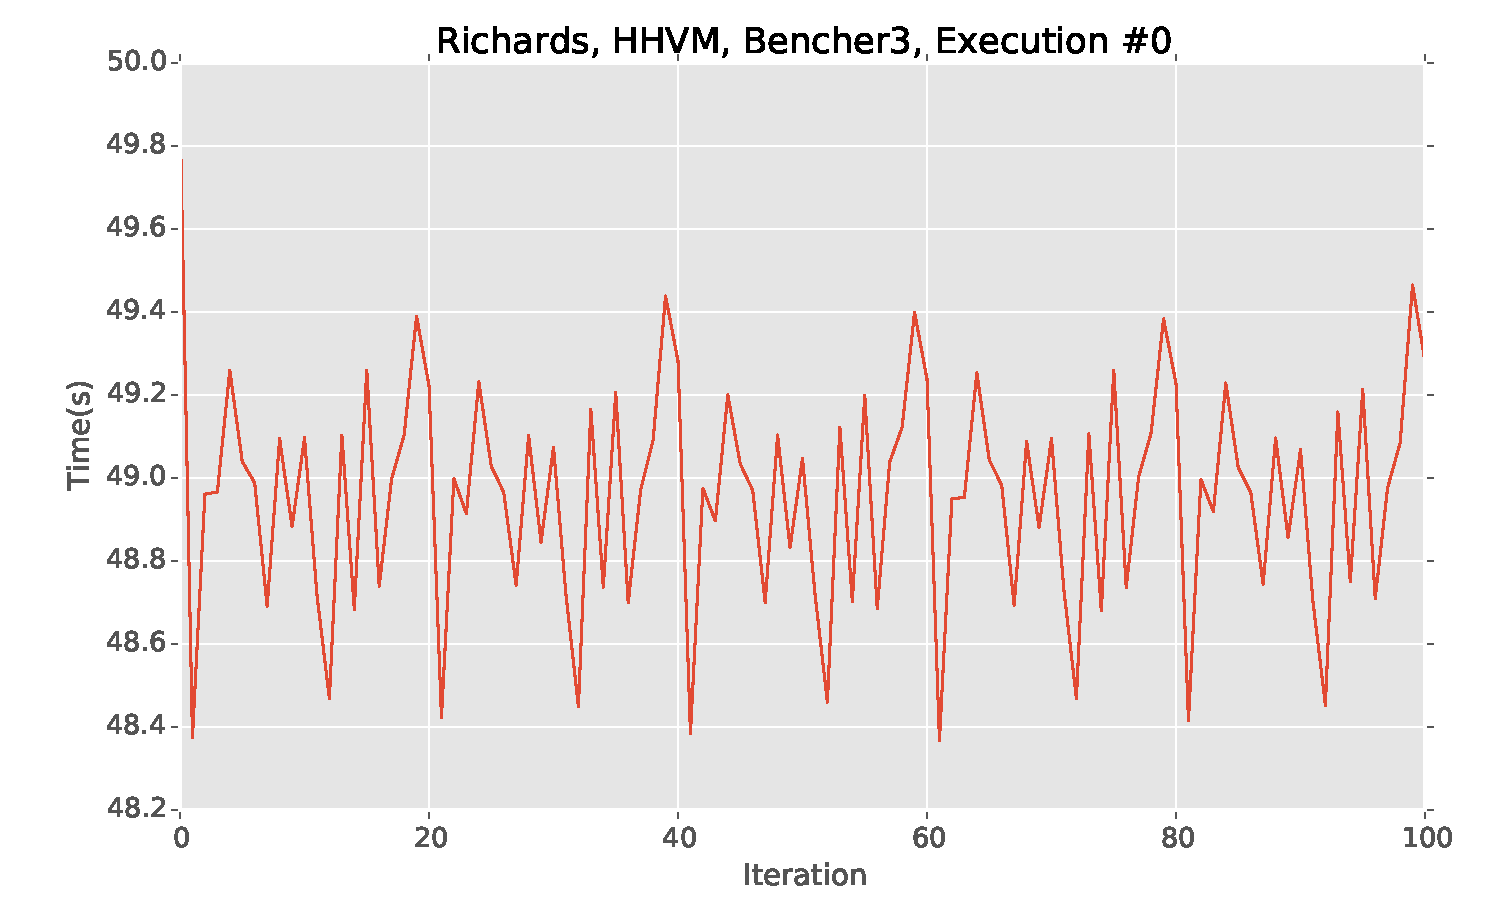
\includegraphics[width=\textwidth]{examples/cycles1}
\end{minipage}
}
\caption{A process execution with cycles of 6 in-process iterations.}
\label{fig:examples:cycles}
\end{figure}

\textbf{Cyclic Behaviour} \label{sub:cyclic}
Some benchmarks exhibit cyclic behaviour, where in-process iteration times
repeat in a predictable pattern. We observed varying cycle lengths (the
shortest of length 2, ranging up to several hundred): the example in
Figure~\ref{fig:examples:cycles} shows an example with a cycle of 6 in-process
iterations.


\begin{figure}[tbp]
\makebox[\textwidth][c]{
\begin{minipage}{.65\textwidth}
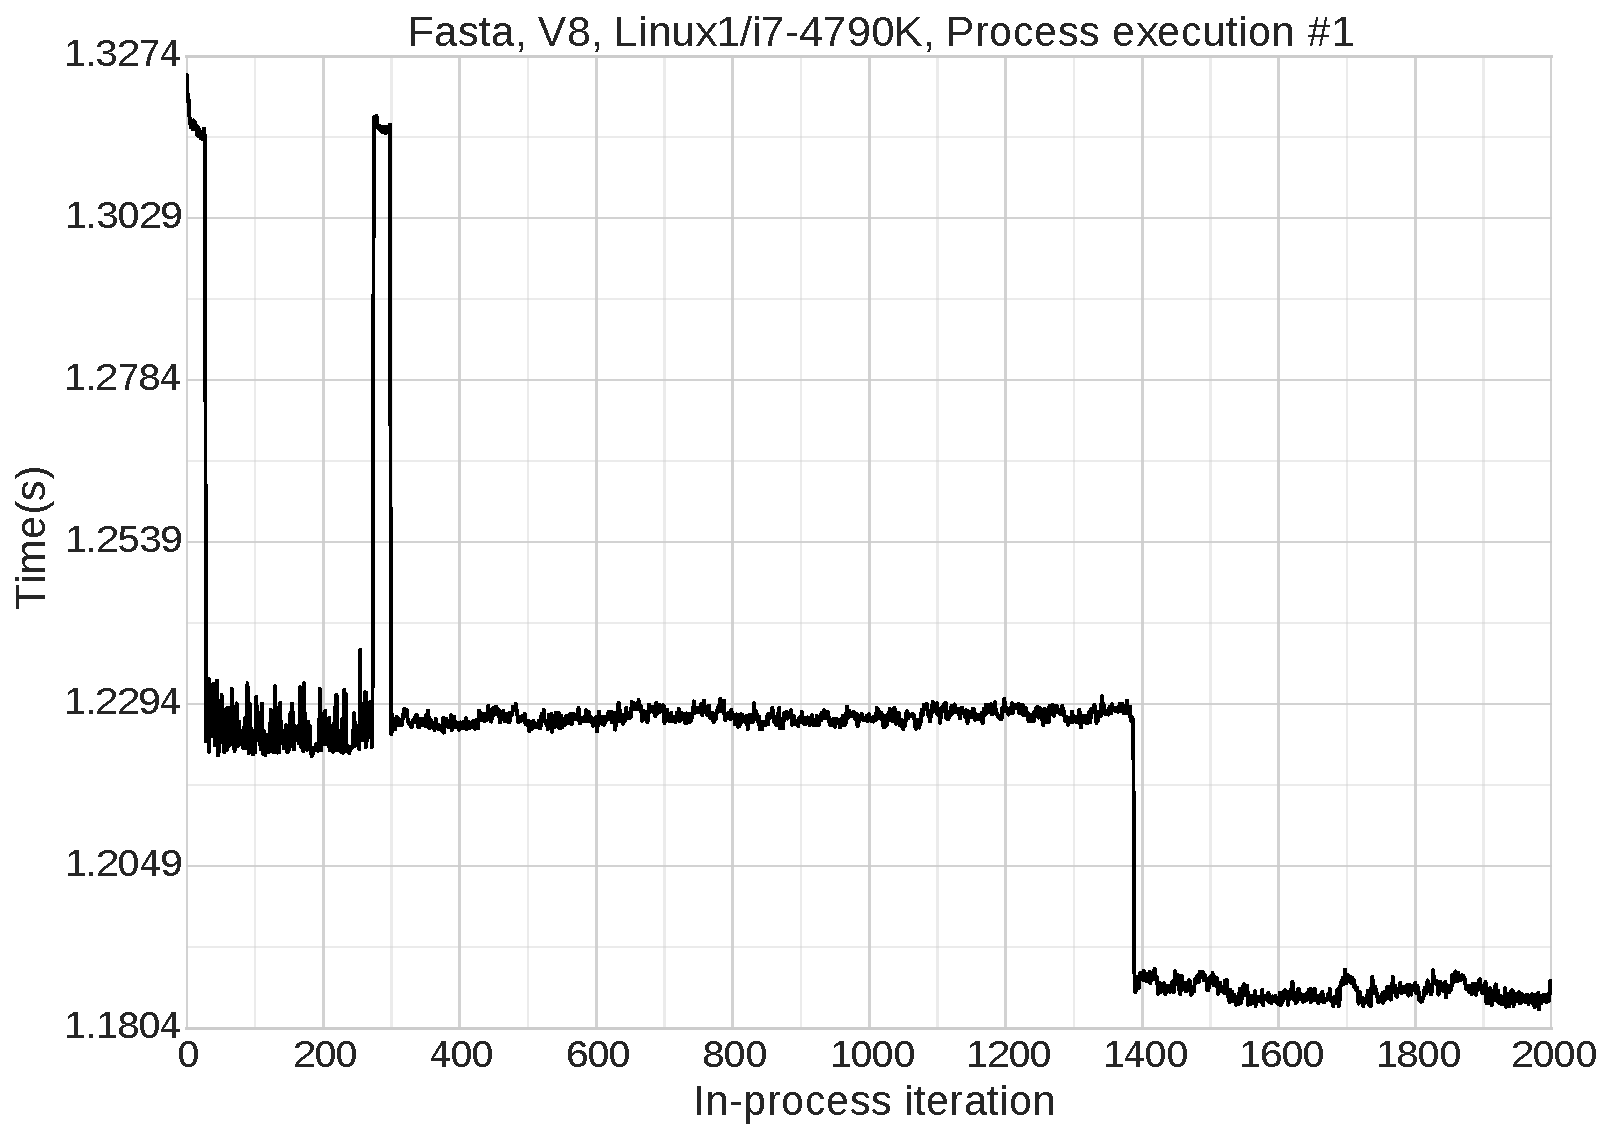
\includegraphics[width=\textwidth]{examples/slow_warmup1}
\end{minipage}
}
\caption{An example of a late phase change, in a definite speed-up occurring
at in-process iteration \#1387.}
\label{fig:examples:late1}
\end{figure}

\textbf{Late Phase Change} \label{sub:phase}
Late phase changes are one of the surprising results from our experiment: it is
clear that some benchmarks change phase after a much larger number of in-process iterations
than previous experiments have considered, as shown in Figure~\ref{fig:examples:late1}.
It is important to note that `late' is relative only to the number of in-process
iterations we ran in our experiment: it is probable that some benchmarks would
undergo further phase changes if we were to run a greater number of in-process
iterations. Note that late phase changes are orthogonal to most of our other
classifiers: after a late phase change, a benchmark may run faster, slower, or
become cyclic etc.


\begin{figure}[tbp]
\makebox[\textwidth][c]{
\begin{minipage}{.65\textwidth}
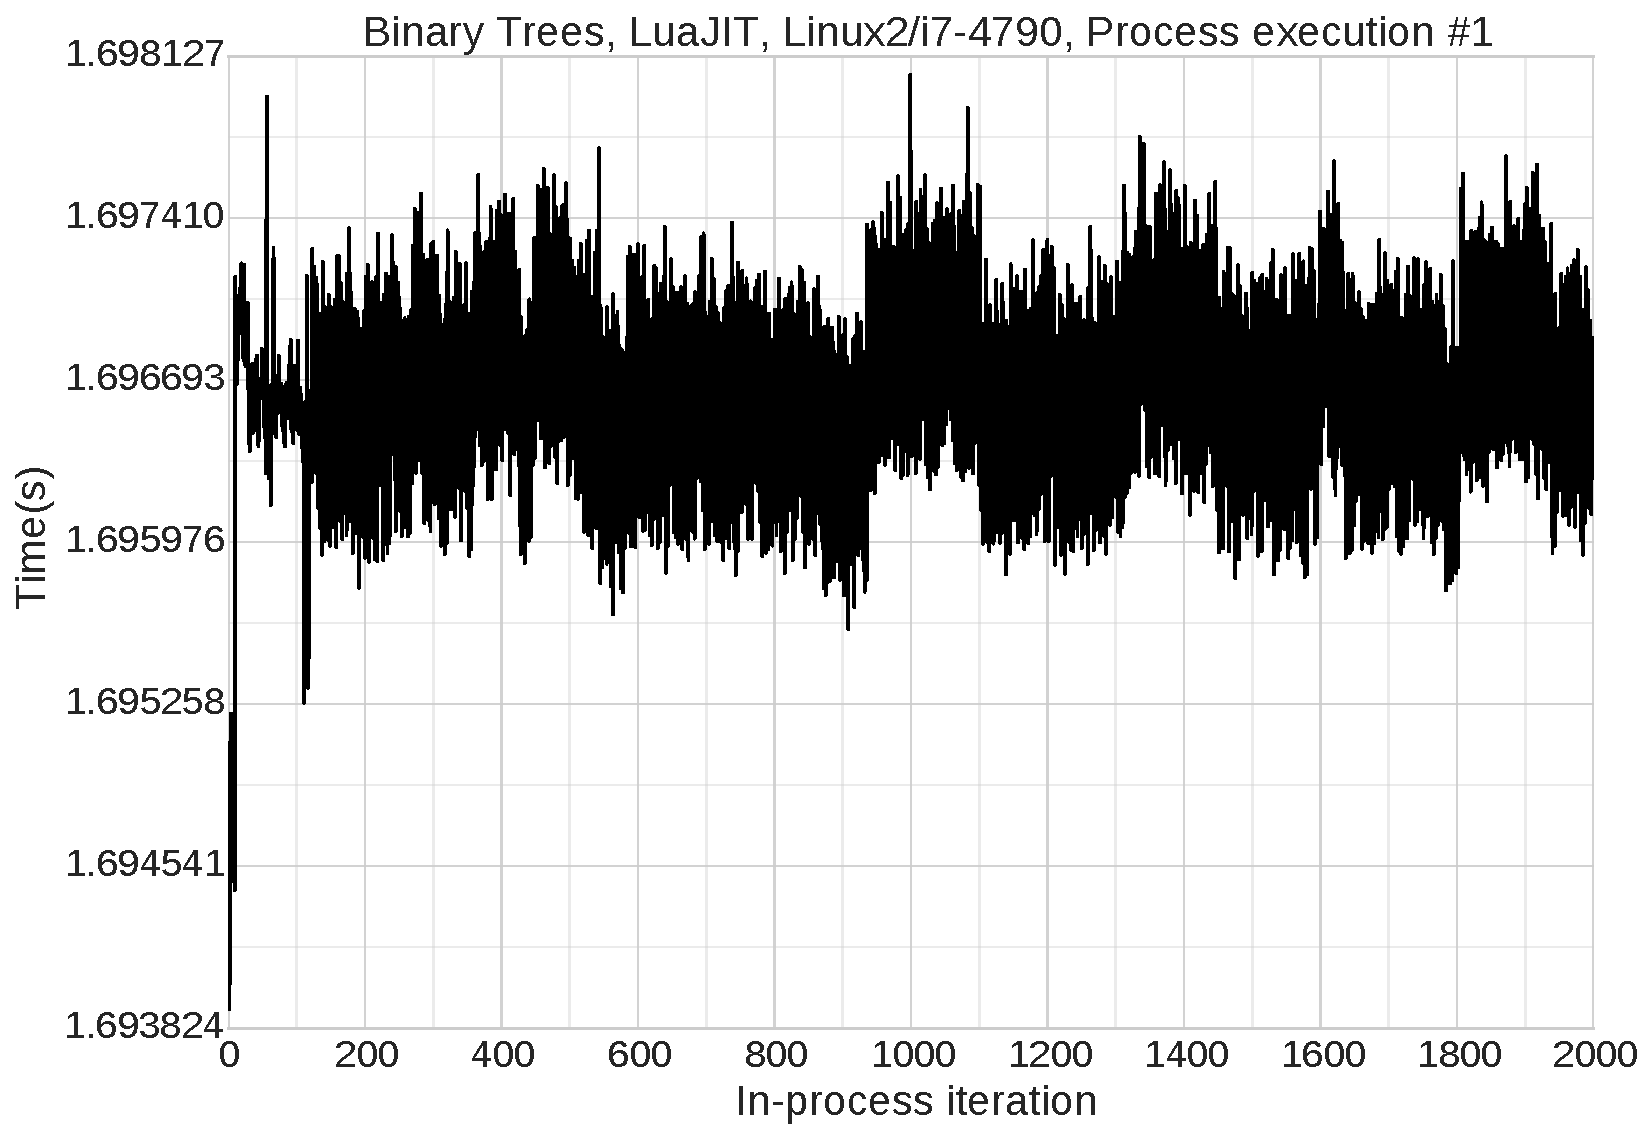
\includegraphics[width=\textwidth]{examples/many_phases}
\end{minipage}
}
\caption{An example of never-ending phase changes.}
\label{fig:examples:neverending}
\end{figure}

\textbf{Never-ending Phase Changes} \label{sub:long}
Some benchmarks keep changing phase without appearing to finally settle on a
single phase. Note that sometimes this can involve cycling between a small
number of phases, or moving between a seemingly arbitrary number of different
phases (as shown in Figure~\ref{fig:examples:neverending}).


\begin{figure*}[p]
\makebox[\textwidth][c]{
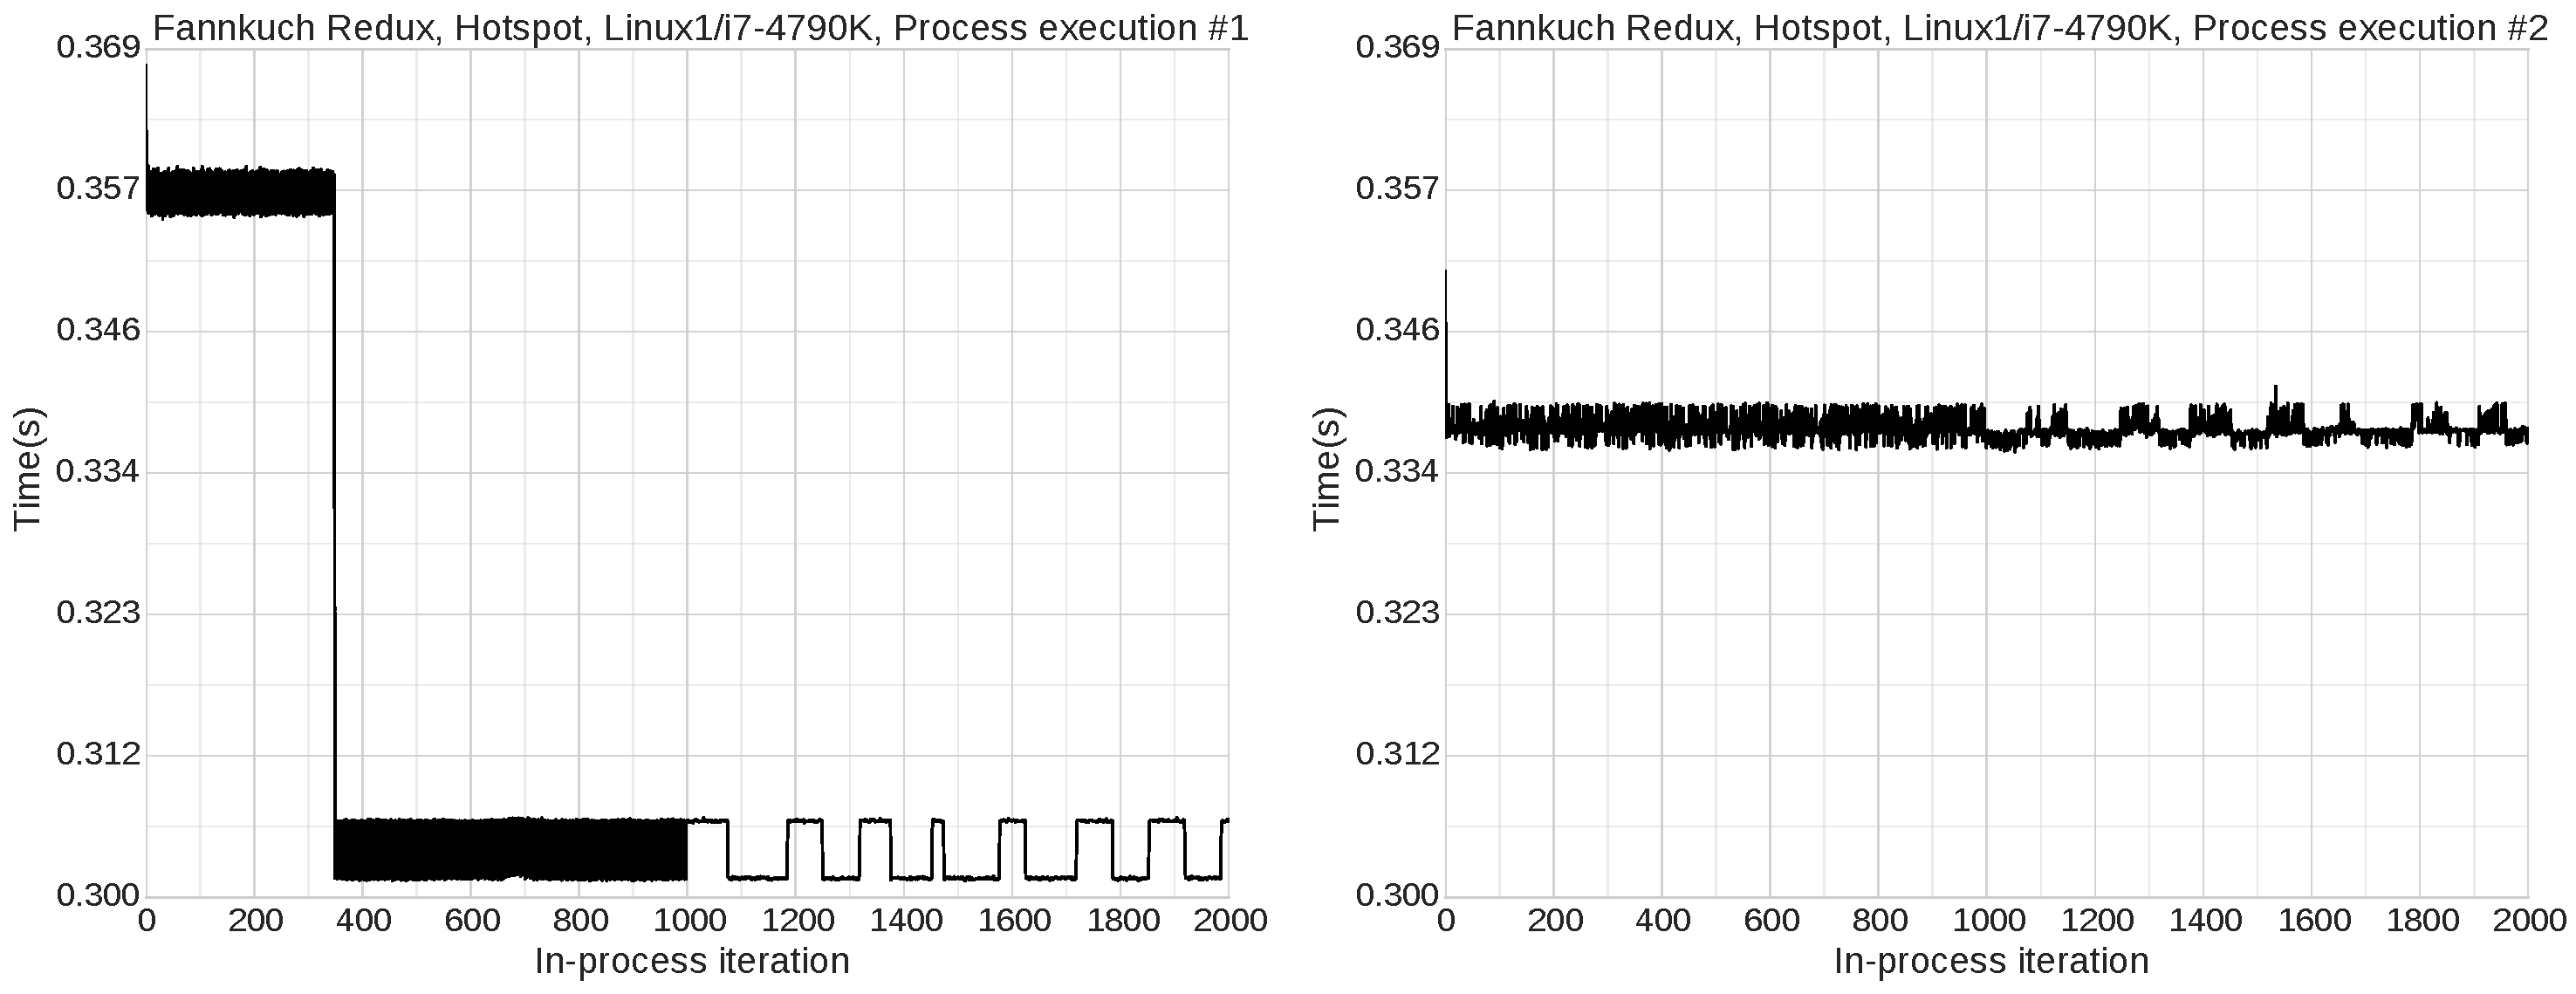
\includegraphics[width=1.3\textwidth]{examples/inconsistent1.pdf}\\
}
\makebox[\textwidth][c]{~}  % only way I could add vertical space
\makebox[\textwidth][c]{
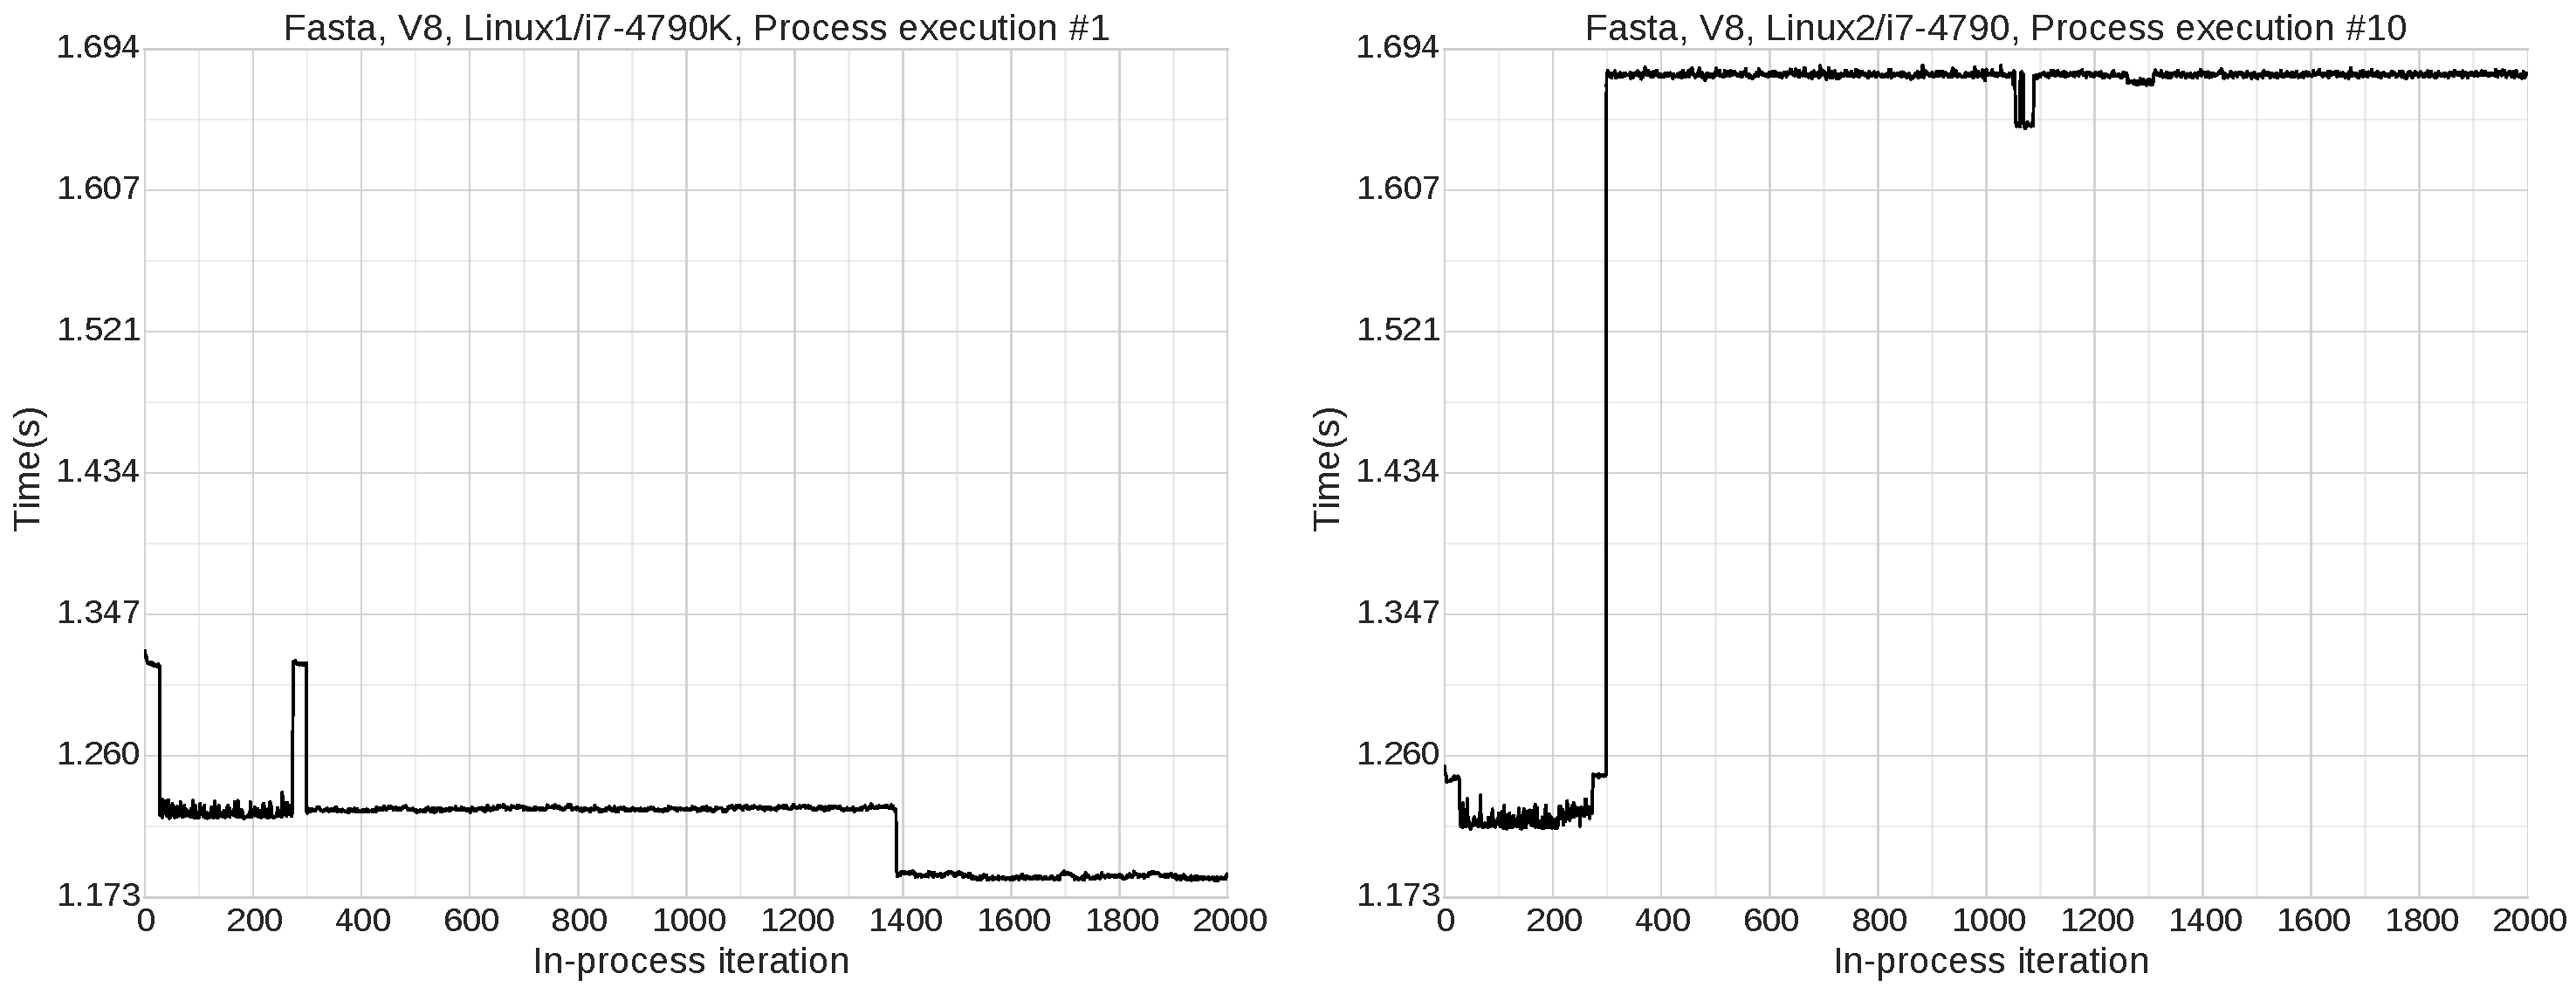
\includegraphics[width=1.3\textwidth]{examples/inconsistent2.pdf}
}
\caption{Examples of inconsistent benchmarks.
The top row shows inconsistencies between different process
executions on the same machine. In this case the Fannkuch Redux benchmark
seems to follow two distinct patterns on different process executions,
sometimes going through a second warmup phase until around in-process iteration 375, and
other times not doing so (based on our data, these two patterns seem to occur
equally often). The bottom row shows inconsistencies between
machines.}
\label{fig:examples:inconsistent}
\end{figure*}

\textbf{Inconsistent} \label{sub:inconsistent}
A number of benchmarks behave inconsistently when comparing different process executions. Sometimes this occurs on
in-process executions within a single machine; sometimes only across machines.
Figure~\ref{fig:examples:inconsistent} shows examples of both cases.


\section{Threats to Validity}
\label{sec:threats}

While we have designed our experiment as carefully as possible, we do not
pretend to have controlled every possibly confounding variable. Indeed, our
experience when designing the experiment has been one of gradually uncovering
confounding variables whose existence we had not previously imagined. It
is inevitable that there are further confounding variables that we
do not know about; some of these may be controllable, although many may not be.
It is possible that currently confounding variables we are not aware of have
coloured all our results.

We have tried to gain a partial understanding of the effects of different
hardware on benchmarks by using benchmarking machines with the same OS but
different hardware. However, while the hardware between the two is
different, much more distinct hardware (e.g.~using a non-x86 architecture) is
available, and is more likely to uncover hardware-related differences.
However, hardware cannot always be controlled in isolation from software:
the greater the differences in hardware, the more likely that JIT compilers
compilers are to use different code paths (e.g.~different code generators and
the like). Put another way, an apples-to-apples comparison across very different
hardware is likely to be impossible, because the software being run will
change its behaviour.

We have not yet systematically tested whether rebuilding VMs effects warmup, an
effect noted by \kalibera. Our previous experience of JIT compilers suggests
that there is little effect in rebuilding such VMs when measuring peak
performance~\cite{barrett15approaches}. However, since measuring warm-up largely
involves measuring code that was not created by a JIT compiler, it is possible
that these effects may impact upon our experiment. To a very limited extent, the
rebuilding of VMs that occurred on our different VMs gives some small evidence
as to this effect, or lack thereof, but we will perform a deeper investigation
in the future.

The checksums we added ensure that, at a user-visible level, each benchmark
performs equivalent work in each language variant. However, it is impossible to
say whether each performs equivalent work at the lowest level or not. For
example, choosing to use a different data type in a language's core library may
substantially impact performance. There is also the perennial problem as to the
degree to which an individual language benchmark should maintain the structure
of other language's implementations: a benchmark for a given language could be
rewritten in a way that betters either or both of its warmup and peak
performance. From our perspective, this possibility is somewhat less important,
since we are more interested in the warmup patterns of reasonable programs,
whether they be the fastest possible or not. It is also possible that by
inserting checksums we have created unrepresentative benchmarks, though
this complaint could arguably be directed at the unmodified benchmarks too.

Although \krun does as much to control CPU clock speed as possible, modern CPUs
do not always respect operating system requests. Even on Linux, where we control
the CPU's P-state, we cannot guarantee that this fixes the CPU frequency: as
the Linux kernel documentation states, ``the idea that frequency can be set to a single
frequency is fiction for Intel Core processors''~\cite{pstate}. In
some cases, changes the CPU makes to its performance are detected and reported
by the operating system (e.g.~performance throttling due to potential
overheating); in other cases, changes may go undetected or unreported.
Despite this, our benchmarks show fairly predictable performance across
different hardware, suggesting that the effect of CPU performance changes may
not be significant in our case.

In controlling confounding variables, our benchmarking environment necessarily
deviates from standard configurations. It is possible that in so doing, we have
created a system that shows warmup effects that few people will ever see in
practise.

We have identified a number of different styles of warmup (slowdown, cyclic,
etc.). However, we do not claim to have uncovered all possible warmup styles. It
is quite possible that other patterns exist that either do not show up in our
data, or which we have not detected.


\section{Discussion}
\label{sec:Discussion}

Even though we had a reasonable amount of experience designing and implementing
experiments, the experiment in this paper took more time and effort than we
expected. In part this is because there is limited precedent for such detailed
experiments. Investigating possible confounding variables, understanding how to
control them, and implementing the necessary checks, all took time. In many
cases, we had to implement small programs or systems to understand a variable's
effect (e.g.~that Linux allows a process to allocate memory beyond that
specified in the soft and hard \texttt{ulimit}).

In some cases, we found that seemingly reasonable settings had undesirable
effects. Most notably, we trialled running experiments on a fixed CPU core which
no other processes were allowed to run on (using Linux's \texttt{isolcpus}
feature). While this may have removed noise from some some VMs,
it slowed others down by
a factor of up to 3x. The reason for this is that pinning a process to a CPU
core also pins that processes threads to the same core. Some VMs -- such as
JRuby/Truffle -- create extra threads for compilation, GC, and the like. By
running all these threads on a single core, we removed the considerable
performance benefits of running such computation in parallel.


\section{Related work}

There are two works we are aware of which explicitly note unusual warmup
patterns. Gil et al.'s main focus is on non-determinism over execution runs on
HotSpot, and the difficulties this raise in terms of providing reliable
benchmarking numbers~\cite{gil11microbenchmark}. In this process, they report at
least one benchmark (listBubbleSort) which on some executions undergoes what we
would classify a slowdown. \kalibera note the
existence of what we have called cyclic behaviour (in the context of benchmarking,
they then require the user to
manually pick one part of the cycle for measurement~\cite{kalibera13rigorous}).


\section{Conclusions}
\label{sec:conclusion}

Warmup has always been an informally defined term~\cite{seaton15phd} and in this
paper we have shown cases where that informal definition fails to hold.
To the best of our knowledge, this paper is the first to classify different
`warmup' styles and note the relatively high frequency of non-traditional
classifications such as slowdown and never-ending phase changes.
However, as every keen student of history discovers, it is easier to destroy than to
create: we have not yet found an acceptable alternative definition of warmup.
Based on our experiences thus far, we think it unlikely that the different
styles of warmup we have seen can be captured in a single metric. We suspect it
is more likely that a number of different metrics will be needed to describe and
compare warmup styles.

\bibliographystyle{plain}
\bibliography{bib}


\end{document}

